\documentclass[../main/main.tex]{subfiles}
\graphicspath{{./figures/}}

\makeatletter
\renewcommand{\@chapapp}{Travaux pratiques -- TP}
\renewcommand{\chaplett}{TP}
\makeatother

% \toggletrue{student}
% \toggletrue{corrige}
% \renewcommand{\mycol}{black}
% \renewcommand{\mycol}{gray}

% \usepackage{pdfpages}

\hfuzz=5.003pt

\begin{document}
\setcounter{chapter}{8}

\settype{enon}
\settype{solu_prof}
\settype{solu_stud}

\chapter{\cswitch{Correction du TP}{Dosage par \'etalonnage~: spectrophotom\'etrie et conductim\'etrie}}

\enonce{
	\begin{tcn}[sidebyside, sidebyside align=top](appl)<ctb>"how"'t'{Capacités exigibles}
		\begin{itemize}[label=\rcheck]
			\item Effectuer des tests qualitatifs
			\item Réaliser des dosages par étalonnage.
			\item Proposer ou mettre en œuvre, à partir d’informations fournies, des
			      tests qualitatifs préalables à l’élaboration d’un protocole.
		\end{itemize}
		\tcblower
		\begin{itemize}[label=\rcheck]
			\item Déterminer une concentration en exploitant la mesure de grandeurs
			      physiques caractéristiques de l’espèce ou en construisant et en
			      utilisant une courbe d’étalonnage.
			\item Déterminer une concentration ou une quantité de matière par
			      spectrophotométrie UV-Visible.
		\end{itemize}
	\end{tcn}
	\vspace{-10pt}
	\section{Objectifs}
	\begin{itemize}
		\item Revoir le protocole de dilution (niveau lycée).
		\item Revoir la technique de spectrophotométrie.
		\item Utiliser la loi de \textsc{Beer-Lambert}.
		\item Revoir le protocole expérimental de conductimétrie~;
		\item Utiliser la loi de \textsc{Kohlrausch}.
	\end{itemize}
}

\enonce{%
\section{S'approprier}

\subsection{Le dosage par étalonnage}

Un dosage par étalonnage consiste à déterminer la concentration molaire d'une
espèce chimique en solution en comparant une grandeur physique (conductance,
absorbance…) de la solution avec la même grandeur physique mesurée pour des
solutions étalons (solution dont on connait avec précision la composition). En
supposant qu'il existe une relation entre la valeur de la grandeur physique et
la concentration, on peut alors déterminer la concentration en une espèce
chimique donnée dans la solution inconnue en comparant la valeur de la grandeur
physique pour cette solution avec la valeur de la grandeur physique pour la
solution étalon.

\subsection{Le principe de la spectrophotométrie}

Certaines espèces chimiques sont capables d'absorber la lumière UV ou visible.
Ainsi, est-il possible de relier l'intensité lumineuse transmise à une longueur
d'onde donnée à la concentration d'une espèce en solution par la \textbf{loi de
	Beer-Lambert}~:
\begin{tcb}(prop){Loi de \textsc{Beer-Lambert}}
	\[\boxed{A = \log\left(\frac{I_0}{I}\right) = \sum_{i=1}^{N}\epsilon_i \,
			\ell \, c_i}\]
	Avec~:
	\begin{itemize}
		\item $A$ est l'absorbance (adimensionnée). C'est une grandeur
		      \textbf{additive}
		\item $I_0$ l'intensité lumineuse incidente (en $\si{W.m^{-2}}$)
		\item $I$ l'intensité lumineuse en sortie de cuve (en $\si{W.m^{-2}}$)
		\item $\epsilon_i$ le coefficient d'extinction molaire de l'espèce ${\rm
					      X}_i$ à la longueur d'onde $\lambda$ (dépend de l'espèce chimique
		      étudiée mais aussi marginalement du solvant et de la température)
		\item $\ell$ la largeur de la cuve traversée par le faisceau (en $\si{m}$)
		\item $c$ la concentration en l'espèce absorbante $\ce{X}_i$ (en
		      $\si{mol.L^{-1}}$)
	\end{itemize}
\end{tcb}

Ici, on se limite à une unique espèce absorbante, tel que la relation de
Beer-Lambert devient
\[\boxed{A = \log\left(\frac{I_0}{I}\right) = \epsilon \, \ell \, c}\]

La valeur de $\epsilon \, \ell$ est bien souvent inconnue. Pour
obtenir $c_0$ connaissant $A_0$ de notre solution inconnue, il est donc
nécessaire de déterminer préalablement l'expression de la fonction $A=f(c)$.
Cette courbe est appelée \textbf{courbe d'étalonnage}. Elle est obtenue avec
l'ensemble des points de coordonnées $(A_i, c_i)$ obtenus à partir d'un ensemble
de solutions étalons $S_i$ de concentrations connues.

\subsection{Le principe de la conductimétrie}

Cette méthode repose sur l'existence d'ions en solution et sur leur capacité à
faciliter le passage d'un courant. La nature des ions et leurs concentrations
modifient la conductance $G$ du système (grandeur qui est l'inverse de la
résistance $R$) exprimée en \si{S} (Siemens). Plus le milieu est propice au
passage du courant, plus la conductance est élevée. Celle-ci est reliée à trois
paramètres principaux~:

\begin{enumerate}
	\item la conductivité $\sigma$ du système
	\item la longueur $\ell$
	\item la section $S$ de la cellule
\end{enumerate}

La conductance s'exprime alors selon
\[\DS G = \frac{\sigma S}{\ell}\]

Ainsi, on ne parle pas de conductance \cancel{de la solution}, puisque la
conductance dépend de la cellule de mesure et de sa géométrie. L'unité de
conductivité est le $\si{S.m^{-1}}$~; le quotient $K = \ell / S$ est appelé
constante de cellule. Ainsi, on a $G = \sigma / K$. La mesure de la conductance
s'effectue avec un conductimètre, qui est en fait un ohmmètre.\bigbreak

La conductivité $\sigma$ de la solution peut alors s'exprimer par la \textbf{loi
	de Kohlrausch}, exprimée sous une forme avec la charge de l'ion~:
\begin{tcb}(prop){Loi de \textsc{Kohlrausch}}
	\[\boxed{\sigma = \sum_{i} \lambda_i \left|z_i\right| [\ce{X}_i]}\]

	Avec~:
	\begin{itemize}
		\item $\lambda_i$ la conductivité molaire ionique de l'ion $\ce{X}_i$ (en
		      $\si{S.m^2.mol^{-1}}$) donnée dans les tables
		\item $z_i$ la charge de l'ion $\ce{X}_i$
		\item $[\ce{X}_i]$ la concentration de l'ion $\ce{X}_i$
	\end{itemize}
\end{tcb}

\begin{tcn}(impo){Attention}
	\begin{center}
		\bfseries
		La conductivité $\sigma$ de la solution prend en compte tous les ions
		présents dans la solution. Il faut donc faire l'inventaire des ions en
		solution avec soin.
	\end{center}
\end{tcn}

En supposant que l'on ne fait varier que d'une unique espèce ionique (et donc
conductrice) dans la solution, on pourra noter $c = [\ce{X}_i]$ la concentration
de cette espèce. La \textbf{courbe d'étalonnage} est alors la représentation
graphique de $\sigma = f(c)$ obtenue avec l'ensemble des points de coordonnées
$(c_i~; \sigma_i)$ où $\sigma_i$ sont les conductivités des différentes
solutions étalons $S_i$ de concentration $c_i$. Connaissant la conductivité
$\sigma_0$ de la solution $S_0$ inconnue, on en déduit grâce à la courbe
d'étalonnage la concentration molaire $c_0$ de la solution $S_0$.

\subsection{Le principe de la dilution}

\begin{tcb}(prop){Dilution}
	On peut diminuer la concentration $c$ d'une solution de volume $V$ en
	ajoutant du solvant jusqu'à un volume $V'$. La concentration $c'$
	obtenue est alors
	\[\boxed{cV = c'V'}
		\Longleftrightarrow
		\boxed{\frac{c}{c'} = \frac{V'}{V}}
	\]
\end{tcb}

En effet, la quantité de matière de soluté ne change pas avec l'ajout de
solvant, autrement dit $n$ est constant. On a donc
\[ c = \frac{n}{V} \qqet c' = \frac{n}{V'}\]
d'où le résultat.
}

\setcounter{section}{2}
\section{Analyser}

\subsection{Préliminaire sur la solution de permanganate de potassium}

\enonce{%
	Le permanganate de potassium solide $\ce{KMNO4_{\sol}}$, est un antiseptique
	utilisé pour désinfecter des plaies, les fruits ou légumes, traiter les eaux… Il
	se vend en pharmacie sous forme de sachet~: la notice indique que le sachet
	contient $\SI{0.25}{g}$ de $\ce{KMNO4_{\sol}}$ à dissoudre dans $\SI{2.5}{L}$
	d'eau. C'est ainsi qu'une solution aqueuse $S_0$ de permanganate de potassium
	$\ce{K^{+}_{\aqu} + MNO4^{-}_{\aqu}}$ a été obtenue. Il s'agit ici de
	vérifier, par deux méthodes différentes, l'indication de masse portée sur le
	sachet.

	\begin{tcb}(data)<lfnt>{Donnée}
		Masse molaire du permanganate de potassium~: $M = \SI{158,0}{g.mol^{-1}}$.
	\end{tcb}
}

\setlist[blocQR,1]{leftmargin=10pt, label=\clenumi}
\QR{%
	Pourquoi peut-on suivre le dosage du permanganate par spectrophotométrie~?
}{%
	Le permanganate est la seule espèce colorée, permettant de déterminer sa
	concentration par analyse de l'absorption.
}
\QR{%
	\noindent
	\begin{minipage}[t]{.58\linewidth}
		Sur l'étiquette du permanganate de potassium, on peut voir ces
		pictogrammes~: que signifient-ils~? quelles précautions faut-il prendre~?
		Vous pourrez consulter
		\url{http://www.inrs.fr/media.html?refINRS=ED\%204406}
	\end{minipage}
	\hfill
	\begin{minipage}[t]{.40\linewidth}
		~
		\vspace{-15pt}
		\begin{center}
			
\includegraphics[width=\linewidth]{picto3}
		\end{center}
	\end{minipage}
}{%
	C'est un \textbf{comburant}, une espèce nocive ou irritante, et un polluant
	dangereux pour l'environnement.
	\smallbreak
	Il faut donc l'écarter de substances combustibles, éviter tout contact avec
	le corps humain (grâce à des lunettes de protection, des gants, une blouse
	et une hotte), et ne pas la jeter dans n'importe quel évier.
}

\subsection{Préparation des solutions aqueuses étalon}

\enonce{%
	On dispose d'une solution-mère aqueuse $S_1$ de permanganate de potassium de
	concentration molaire $c_1 = \SI{1.00e-3}{mol.L^{-1}}$. On veut préparer, à
	partir de cette solution $S_1$, par dilution, quatre solutions-filles $S_2$ à
	$S_5$ de volume $V = \SI{50.0}{mL}$ et de concentrations molaires $c_2$ à $c_5$.
}

\QR{%
	Compléter le tableau ci-dessous~:
	\begin{center}
		\renewcommand{\arraystretch}{1.3}
		\begin{tabularx}{\linewidth}{|Y|*{4}{|Y}|}\hline
			$S_i$                     &
			$S_2$                     &
			$S_3$                     &
			$S_4$                     &
			$S_5$
			\\\hline
			$c_i$ ($\si{mol.L^{-1}}$) &
			$c_2 = \num{2.00e-4}$     &
			$c_3 = \num{4.00e-4}$     &
			$c_4 = \num{6.00e-4}$     &
			$c_5 = \num{8.00e-4}$
			\\\hline
			$V_i (\si{mL})$           &
			                          &
			                          &
			                          &
			\\\hline
		\end{tabularx}
	\end{center}
}{%
	\leavevmode\vspace*{-15pt}\relax
	\begin{center}
		\renewcommand{\arraystretch}{1.3}
		\begin{tabularx}{\linewidth}{|Y|*{4}{|Y}|}\hline
			$S_i$                     &
			$S_2$                     &
			$S_3$                     &
			$S_4$                     &
			$S_5$
			\\\hline
			$c_i$ ($\si{mol.L^{-1}}$) &
			$c_2 = \num{2.00e-4}$     &
			$c_3 = \num{4.00e-4}$     &
			$c_4 = \num{6.00e-4}$     &
			$c_5 = \num{8.00e-4}$
			\\\hline
			$V_i (\si{mL})$           &
			\num{10}                  &
			\num{20}                  &
			\num{30}                  &
			\num{40}                    \\\hline
		\end{tabularx}
	\end{center}
}

\QR{%
	Décrire le protocole expérimental de la préparation de la solution aqueuse
	$S_2$ sans oublier d'expliciter le calcul du volume prélevé de solution
	aqueuse $S_1$ nécessaire à cette préparation.
}{%
	On conserve la quantité de matière pendant la dilution, mais le volume change.
	Pour avoir $V_1$ et $c_2$ à partir de $c_1$, on aura
	\[
		c_1V_1 = c_2V
		\Lra
		\boxed{V_1 = \frac{C_2V}{C_1}}
		\Ra
		\xul{V_1 = \SI{10}{mL}}
	\]
	\begin{enumerate}
		\item Verser le contenu du grand récipient de solution $S_1$ dans le bécher
		      devant.
		\item En verser une \textbf{petite quantité} dans un bécher personnel,
		      labellé $S_1$.
		\item Revenir à la paillasse, et prélever \SI{10}{mL} de cette solution avec
		      une pipette jaugée.
		\item Insérer les \SI{10}{mL} dans la fiole jaugée de \SI{50}{mL}.
		\item Remplir d'eau distillée jusqu'au trait de jauge, puis mélanger.
	\end{enumerate}
}

\section{Réaliser et valider}

\enonce{%
	\begin{tcb}[bld, cnt](impo)"bomb"{Protection en TP}
		Le port de la blouse fermée et des lunettes est obligatoire durant
		l'ensemble du TP. Les cheveux longs doivent être attachés.
	\end{tcb}

	\subsection{Préparation de la solution fille $S_2$}

	\begin{tcb}(expe){}
		En suivant le protocole que vous avez établi dans la partie Analyser, préparer
		la solution fille $S_2$, \textit{et uniquement la solution $S_2$}.
	\end{tcb}

	\subsection{Dosage par spectrophotométrie}
	\subsubsection{Choix de la longueur d'onde de travail}

	Nous allons dans un premier temps établir le spectre d'absorption du
	permanganate de potassium.

	\begin{tcb}(expe)<itc>{Spectre d'absorption}
		\begin{itemize}
			\item[b]{Calibration du spectrophotomètre}~:
			      \begin{enumerate}
				      \item Calibrer~; Appuyer sur \boxed{0/1} puis \texttt{cuve vide~?}~:
				            \fbox{\texttt{VAL}}. et \texttt{imprimer~?}~: \fbox{\texttt{ESC}}.
				      \item Quand le calibrage est terminé~: le spectro affiche~:
				            \texttt{absorbance}, etc
				      \item Arrêter l'appareil~: \boxed{0/1}.
			      \end{enumerate}
			\item[b]{Redémarrer le spectrophotomètre sous contrôle de l'ordinateur}~:
			      \begin{enumerate}
				      \item Ouvrir Regressi
				      \item Dans Fichier $\ra$ nouveau choisir S250
				      \item Choisir dans le menu du spectro le protocole de communication~:
				            \textbf{S 250 I/PC}.
				      \item Cliquer sur le bouton correspondant au spectro éteint. Le spectro se
				            rallume alors (il faut quelques secondes~!).
			      \end{enumerate}
			\item[b]{Tracé des spectres}~: \texttt{spectre paramétrable $\SIrange{335}{900}{nm}$}~:
			      \begin{enumerate}
				      \item Choisir des longueurs d'ondes variant de $400$ à $\SI{700}{nm}$ avec
				            un pas de $\SI{6}{nm}$.
				      \item Effectuer le zéro avec une cuve remplie d'eau distillée en cliquant
				            sur \texttt{BLANC}. Le spectro trace une ligne (bleue) de zéro pour
				            toutes les longueurs d'ondes.
				      \item Puis réaliser le spectre du permanganate de potassium en remplissant
				            la cuve au $3/4$ de sa hauteur avec la solution $S_3$, puis en
				            cliquant sur \texttt{SPECTRE}.
			      \end{enumerate}
		\end{itemize}
	\end{tcb}

	\begin{tcb}[cnt, bld](impo){Manipulation des cuves}
		\begin{itemize}
			\item Vous prendrez soin de placer les cuves dans le bon sens (face transparente
			      dans le passage du faisceau lumineux), en évitant de poser vos doigts sur les
			      faces par lesquelles le faisceau passe.
			\item
			      Il faut utiliser la même cuve pour \textbf{toutes} vos
			      mesures au spectrophotomètre. Il faut alors la rincer à chaque fois.
		\end{itemize}
	\end{tcb}

	\begin{tcb}(expe)<itc>{Exploitation du graphe}
		\begin{enumerate}
			\item Basculer dans Regressi~: clic sur \texttt{Sauver} et \texttt{Vers
				      régressi} du logiciel du spectro, et remplir le nom de la grandeur
			      ($A$).
			\item Grâce au réticule, pointer la longueur d'onde de la valeur maximale.
		\end{enumerate}
	\end{tcb}
}

\resetQ
\setlist[blocQR,1]{leftmargin=10pt, label=\sqenumi}
\QR{%
	Imprimer la courbe après avoir retiré le zéro en $x$ et relié les points
	grâce à un lissage d'ordre 3 (dans le menu \texttt{Coordonnées}, décocher
	«~zéro inclus~»).
}{%
	\begin{center}
		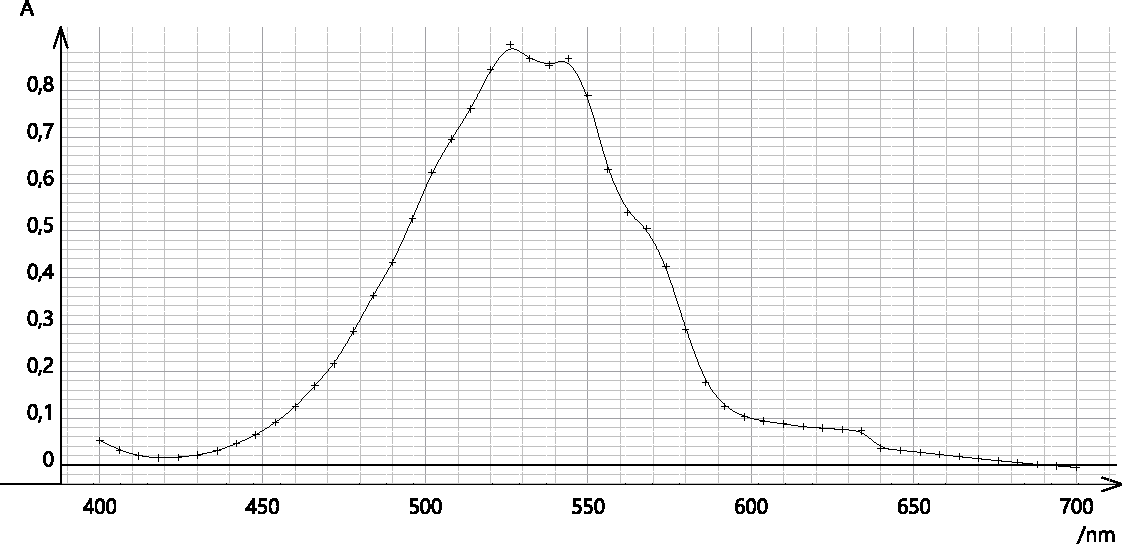
\includegraphics[width=.8\linewidth]{absorbance}
		\captionof{figure}{Résultat de Regressi.}
		\label{fig:absorbance}
	\end{center}
}
\QR{%
	À quelle longueur d'onde doit-on travailler ensuite pour avoir un maximum de
	précision sur la mesure de l'absorbance~? Indiquer le tracé sur vos courbes
	imprimées.
}{%
	Pour augmenter la précision de l'appareil et limiter l'incertitude sur les
	mesures, on se place à la longueur d'onde pour laquelle le coefficient
	d'absorption molaire de la substance est maximum.
}

\setcounter{subsection}{2}
\setcounter{subsubsection}{1}
\subsubsection{Tracé de la courbe d'étalonnage}

\enonce{%
	% \begin{tcb}[cnt](impo){Attention}
	% \end{tcb}
	%
	\begin{tcb}(expe)<itc>{Tracé de la courbe d'étalonnage}
		\begin{enumerate}
			\item Déconnecter le spectrophotomètre de l'ordinateur en le débranchant
			      salement (mais proprement), puis le rallumer manuellement. Suivez
			      les instructions~: il vous donnera alors les mesures.
			\item Le spectrophotomètre va de nouveau se calibrer.
			\item Choisir la longueur d'onde de travail~: $\lambda = \cswitch{%
					      \SI{526}{nm}
				      }{%
					      ……… \si{nm}
				      }%
			      $.
			\item Pour une solution d'eau distillée (ou «~blanc~»), fixer $A = 0$.
		\end{enumerate}
	\end{tcb}
}

\QR{%
	Mesurer l'absorbance de chacune des solutions réalisées et compléter
	le tableau suivant~:
	\begin{center}
		\renewcommand{\arraystretch}{1.3}
		\begin{tabularx}{\linewidth}{|Y*{6}{|Y}|}\hline
			Solution               & $S_2$     & $S_3$     & $S_4$     & $S_5$     & $S_1$ & $S_0$
			\\\hline
			$c (\si{mmol.L^{-1}})$ &
			\num{0.2}              & \num{0.4} & \num{0.6} & \num{0.8} & \num{1.0} &
			\\\hline
			A                      &
			                       &           &           &           &           &
			\\\hline
		\end{tabularx}
	\end{center}
}{%
	On relève $\lambda\ind{max} \approx \SI{526}{nm}$. On rentre cette valeur sur
	le spectrophotomètre.
	\begin{center}
		\renewcommand{\arraystretch}{1.3}
		\begin{tabularx}{\linewidth}{|Y*{6}{|Y}|}\hline
			Solution               &
			$S_2$                  &
			$S_3$                  &
			$S_4$                  &
			$S_5$                  &
			$S_1$                  &
			$S_0$
			\\\hline
			$c (\si{mmol.L^{-1}})$ &
			\num{0.2}              &
			\num{0.4}              &
			\num{0.6}              &
			\num{0.8}              &
			\num{1.0}              &
			\num{0.60}
			\\\hline
			A                      &
			\num{0.492}            &
			\num{0.903}            &
			\num{1.313}            &
			\num{1.729}            &
			\num{2.2}              &
			\num{1.391}
			\\\hline
		\end{tabularx}
	\end{center}
}

\QR{%
	Sur votre session, dans Régressi ou Latispro au choix, tracer la
	courbe $A = f(c)$. La modéliser par une fonction linéaire. Cette droite
	est aussi appelée «~échelle de teinte~». L'imprimer.
}{%
	% \begin{figure}[htbp]
	%   \centering
	%   \includegraphics[width=.5\linewidth]{}
	%
	%   \caption{}
	%   \label{fig:}
	% \end{figure}
}

\QR{%
	Vos mesures peuvent-elles être décrites par la loi de
	\textsc{Beer-Lambert}~? Justifier votre réponse \textbf{précisément}.
}{%
	Oui, c'est bien une solution avec une unique espèce colorée, et elle est
	suffisamment peu concentrée pour avoir une absorbance linéaire en fonction de
	la concentration.
}

\subsubsection{Exploitation de la courbe}

\enonce{%
	Nous allons maintenant utiliser la courbe de calibration préalablement établie
	afin de déterminer la concentration molaire en permanganate de potassium de la
	solution $S_0$ inconnue.
}

\QR{%
	Déterminer la concentration molaire $c_0$ de la solution $S_0$ en
	expliquant votre démarche. Indiquer le tracé sur votre courbe imprimée.
}{%
	On mesure $A_0 = \num{1.391}$. On se reporte alors sur la courbe d'étalonnage,
	et on relève $c_0 = \SI{637e-6}{mmol.L^{-1}}$.
}

\QR{%
	En déduire la masse de permanganate de potassium contenue dans un
	sachet commercial, \textbf{ainsi que son incertitude}.
}{%
	\leavevmode\vspace*{-15pt}\relax
	\begin{gather*}
		\boxed{m_0 = c_0MV}
		\qav
		\left\{
		\begin{array}{rcl}
			c_0 & = & \SI{637e-6}{mol.L^{-1}}
			\\
			M   & = & \SI{158}{g.mol^{-1}}
			\\
			V   & = & \SI{2.5}{L}
		\end{array}
		\right.\\
		\AN
		\xul{
			m_0 = \SI{0.251}{g}
		}
		\\\beforetext{Or,}
		u (m_0) = u (c_0) VM
		\qav
		u (c_0) = \SI{57e-5}{mol.L^{-1}}
		\quad \text{par estimation graphique}
		\\\AN
		\xul{u (m_0) = \SI{0.020}{g}}
		\\\beforetext{Ainsi,}
		\xul{m_0 = \SI{0.251 \pm 0.020}{g}}
	\end{gather*}
}

\QR{%
	Déterminer l'écart normalisé entre la valeur obtenue et la valeur du
	fabricant. Conclure.
}{%
	\leavevmode\vspace*{-15pt}\relax
	\[
		\boxed{E_N = \frac{\abs{m_0 - m\ind{theo}}}{u (m_0)}}
		\qquad \AN
		\xul{E_N = \num{0.05}} < 2
		\quad \text{donc la mesure et l'annonce sont cohérentes}
	\]
}

\subsection{Dosage par conductimétrie}
\subsubsection{Tracé de la courbe d'étalonnage}

\enonce{%
	La cellule conductimétrique est constituée de deux lames planes, parallèles,
	en platine. Le conductimètre mesure la résistance $R$ ou la conductance $G$ de
	la colonne de solution qui est directement proportionnelle à la conductivité
	$\sigma$ (notre grandeur d'intérêt).
}

\setlist[blocQR,1]{leftmargin=10pt, label=\clenumi}
\QR<[start=5]>{%
	Proposer (par analogie avec le protocole d'étalonnage suivi en
	spectrophotométrie) un protocole permettant d'utiliser la loi de
	\textsc{Kohlrausch} dans le cas d'une solution aqueuse préparée avec un
	unique soluté ionique.
}{%
	On réalise une mesure de la conductivité pour différentes concentrations
	connues, on réalise la régression linéaire correspondante~; on utilise alors
	l'étalonnage précédent pour déterminer la concentration de la solution voulue
	en mesurant sa conductivité.
}

\begin{tcb}(expe)<lfnt>{}
	Le mettre en œuvre.
\end{tcb}
\begin{tcb}(impo){Attention}
	\begin{itemize}
		\item Vous ferez attention à mesurer la conductivité des différentes
		      solutions de la plus diluée à la plus concentrée pour ne pas polluer les
		      solutions avec votre électrode.
		\item La cellule du conductimètre doit être conservée dans un grand bécher
		      contenant de l'eau distillée.
	\end{itemize}
\end{tcb}

\setlist[blocQR,1]{leftmargin=10pt, label=\sqenumi}
\QR<[start=9]>{%
	Présenter vos conclusions dans un tableau de valeurs.
}{%
	\leavevmode\vspace*{-15pt}\relax
	\begin{center}
		\renewcommand{\arraystretch}{1.3}
		\begin{tabularx}{\linewidth}{|Y*{6}{|Y}|}\hline
			Solution                         &
			$S_2$                            &
			$S_3$                            &
			$S_4$                            &
			$S_5$                            &
			$S_1$                            &
			$S_0$
			\\\hline
			$c (\si{mmol.L^{-1}})$           &
			\num{0.2}                        &
			\num{0.4}                        &
			\num{0.6}                        &
			\num{0.8}                        &
			\num{1.0}                        &
			\num{0.60}
			\\\hline
			$\sigma (\si{\micro S.cm^{-1}})$ &
			\num{27.04}                      &
			\num{46.9}                       &
			\num{72.6}                       &
			\num{95.0}                       &
			\num{121.0}                      &
			\num{75.5}
			\\\hline
		\end{tabularx}
	\end{center}
}

\subsubsection{Exploitation de la courbe d'étalonnage}

\setlist[blocQR,1]{leftmargin=10pt, label=\clenumi}
\QR<[start=6]>{%
	Proposer un protocole permettant de déterminer la concentration molaire de la
	solution $S_0$. Vous expliciterez clairement votre démarche.
}{%
	On mesure $\sigma_0 = \SI{75.5}{\micro S.cm^{-1}}$. On se reporte alors sur la
	courbe d'étalonnage, et on relève $c_0 = \SI{613e-3}{mmol.L^{-1}}$.
}

\begin{tcb}(expe)<lfnt>{}
	Le mettre en œuvre et imprimer si nécessaire.
\end{tcb}

\setlist[blocQR,1]{leftmargin=10pt, label=\sqenumi}
\QR<[start=10]>{%
	En déduire la masse de permanganate de potassium contenue dans un sachet,
	\textbf{ainsi que son incertitude}.
}{%
	Comme précédemment, on obtient
	\[
		\xul{m_0 = \SI{0.242 \pm 0.020}{g}}
	\]
}

\QR{%
	Déterminer l'écart normalisé sur la mesure et conclure.
}{%
	Idem~:
	\[
		E_N = \num{0.4} < 2
	\]
	Les deux valeurs sont bien compatibles.
}

\section{Conclure}

\QR{%
	Laquelle des deux méthodes vous semble-t-elle la plus précise pour ce dosage~?
}{%
	Sur cette mesure, la conductimétrie a donné un résultat moins précis~;
	cependant, il n'est pas clair de conclure quant à la précision de la méthode
	précisément~: une seule expérience ne peut remplacer une étude sérieuse.
}

% \section{Complément~: fiche sécurité}
%
% \subsection{Comburant}
%
% \begin{minipage}{0.77\linewidth}
% 	Substances facilitant les combustions. Les substances comburantes peuvent
% 	embraser des produits combustibles et/ou amplifier un feu existant, rendant
% 	ainsi son extinction difficile.\bigbreak
%
% 	\textbf{PRÉCAUTIONS}
% 	Une substance comburante n'est pas forcement dangereuse en soit. Elle n'est
% 	pas inflammable, mais c'est elle qui permet à un composé inflammable de
% 	brûler. De ce fait, une substance comburante ne doit jamais être conservée à
% 	proximité de substances combustibles.
% \end{minipage}
% \begin{minipage}{0.23\linewidth}
% 	\begin{center}
% 		
\includegraphics[width=\linewidth]{comburant}
% 	\end{center}
% \end{minipage}
%
% \subsection{Nocif (Nn) ou irritant (Xi)}
%
% \begin{minipage}{0.77\linewidth}
% 	Substance pouvant donner lieu à des risques d'atteinte à la santé moins
% 	importants que les substances toxiques et pouvant provoquer une somnolence,
% 	des allergies, des vertiges ou encore pouvant irriter la peau, les yeux et
% 	les voies respiratoires.\bigbreak
%
% 	\textbf{PRÉCAUTIONS}
%
% 	Un tel produit ne doit pas être inhalé ou ingéré. Il ne doit pas entrer en
% 	contact avec la peau ou les yeux. Il est impératif d'éviter tout contact
% 	avec le corps humain. Le non respect de ces consignes peut entraîner la
% 	possibilité de dommages irréversibles par exposition unique, répétée ou
% 	prolongée. Consulter immédiatement un médecin en cas de malaise.
% \end{minipage}
% \begin{minipage}{0.23\linewidth}
% 	\begin{center}
% 		
\includegraphics[width=\linewidth]{nocif}
% 	\end{center}
% \end{minipage}
%
% \medskip
%
% \textbf{ÉQUIPEMENTS OBLIGATOIRES}
% \begin{itemize}
% 	\item Lunettes de protection (même au dessus de lunettes de vue)
% 	\item Gants en latex (selon danger)
% 	\item Blouse en coton
% 	\item Hotte aspirante (selon danger)
% \end{itemize}
%
% \subsection{Polluant}
%
% \begin{minipage}{0.77\linewidth}
% 	Substance dangereuse pour l'environnement.\bigbreak
%
% 	\textbf{PRÉCAUTIONS}
% 	Une telle substance ne doit pas être rejetée dans les eaux usées (lavabo,
% 	wc…). Elle doit être récupérée après utilisation. Contacter une entreprise
% 	chargée de l'élimination des déchets polluants.
% \end{minipage}
% \begin{minipage}{0.23\linewidth}
% 	\begin{center}
% 		
\includegraphics[width=\linewidth]{polluant}
% 	\end{center}
% \end{minipage}
%
% 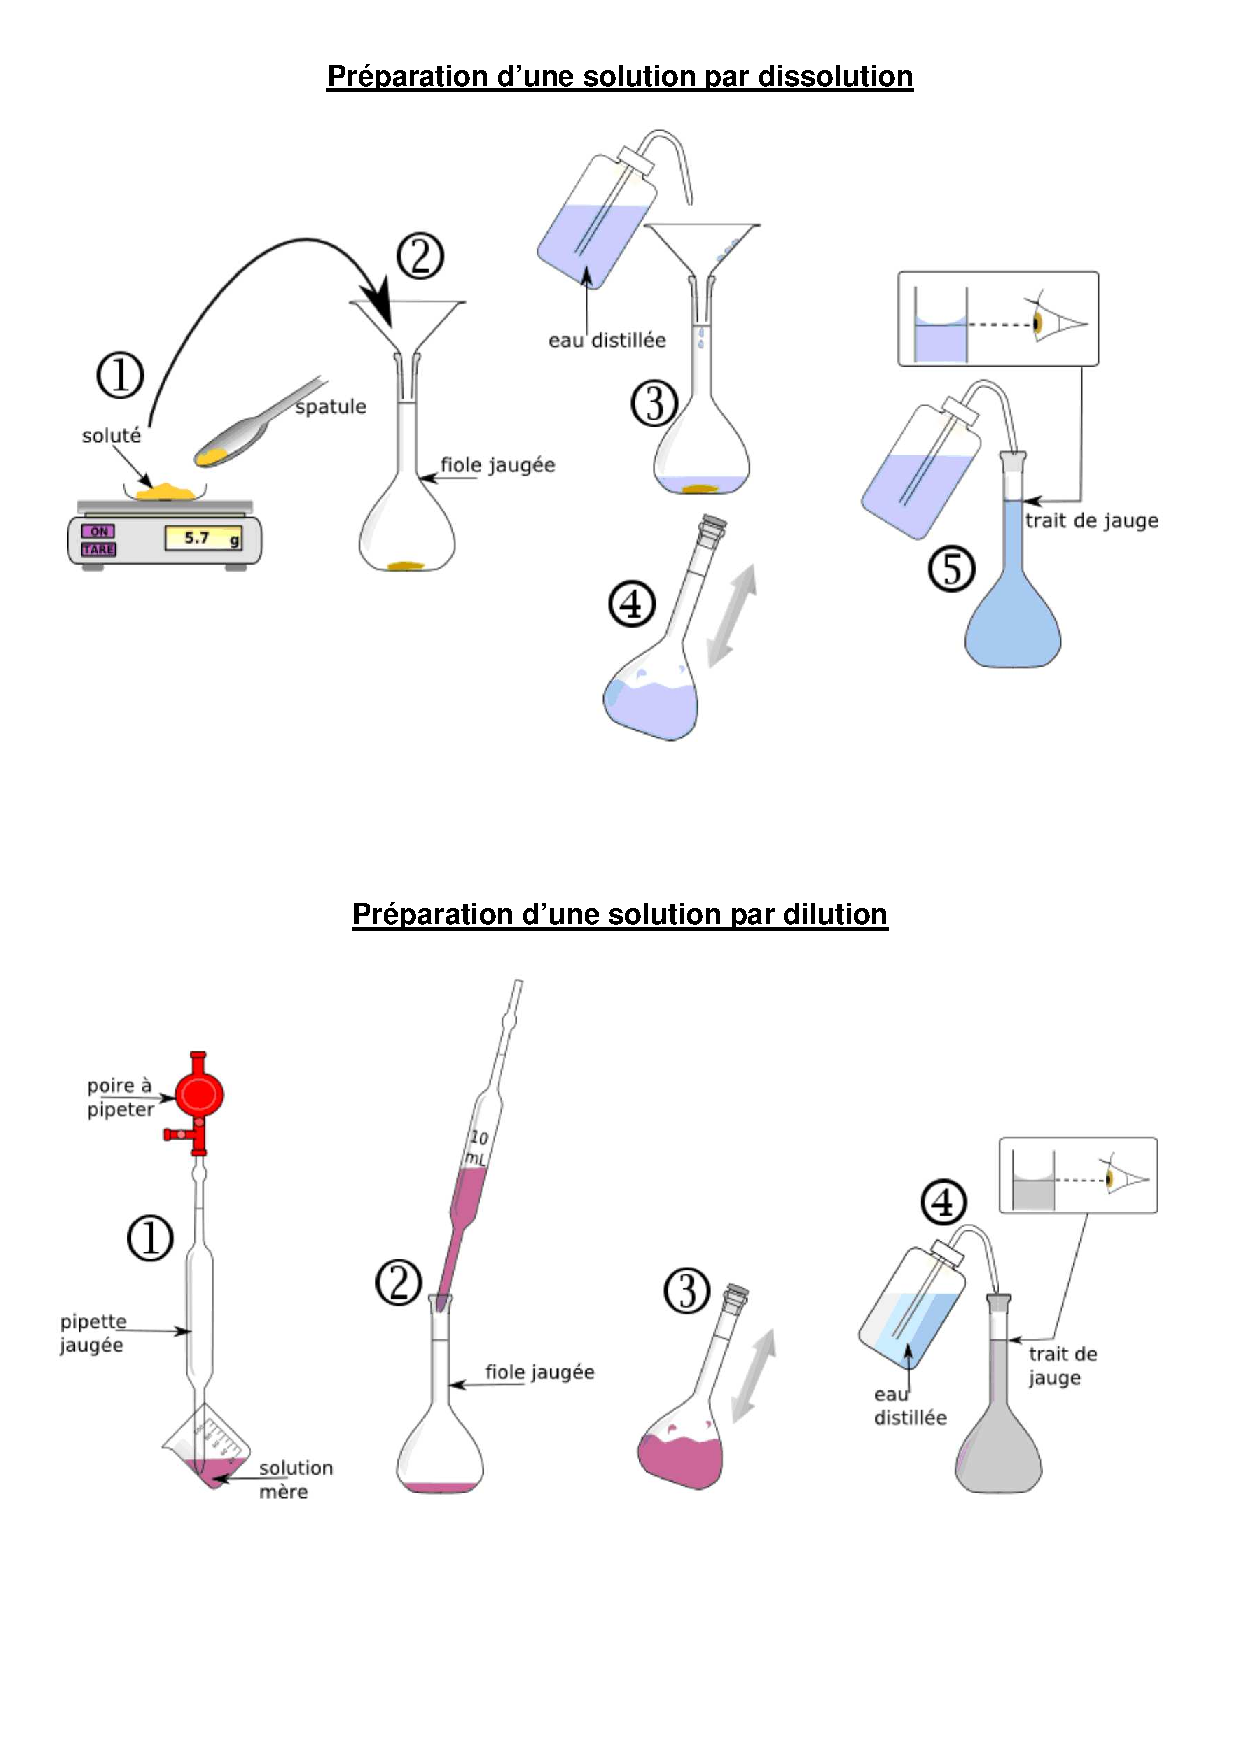
\includepdf[pages={-}]{dissolution_dilution}

\end{document}
